%ju 16-Mai-22 02-Auftragsabwicklung.tex
\section{KFZ-Werkvertrag - Reparaturauftrag /
Werkstattauftrag}\label{kfz-werkvertrag-reparaturauftrag-werkstattauftrag}

\begin{itemize}
\item
  geschäftliche Beziehung zwischen >>Autohaus / Werkstatt<<
  (Auftragnehmer) und dem >>Kunde<< (Auftraggeber)
\item
  Merkmal ist die >>Auftragsnummer<<
\item
  gesetzliche Regelung (Werkvertragsrecht)

  \begin{itemize}
  \item
    \emph{§631} (BGB) Autohaus verpflichtet sich zur Reparatur, Wartung

    \begin{itemize}
    \item
      Erfolg geschuldet
    \end{itemize}
  \item
    \emph{§632} (BGB) Kunde verpflichtet sich zur Entrichtung der
    vereinbarten Vergütung, Werklohn

    \begin{itemize}
    \item
      Kunde muss zahlen, auch wenn über Preise nicht gesprochen wurde,
      aber keine Wucherpreise
    \end{itemize}
  \item
    \emph{§633 Absatz 1} (BGB) Autohaus schuldet Arbeitserfolg, trägt
    Risiko

    \begin{itemize}
    \item
      nach Reparatur oder Umbauten muss Fahrzeug benutzbar, technisch
      einwandfrei sein
    \end{itemize}
  \end{itemize}
\end{itemize}

\textbf{Wichtige Punkte - Reparaturauftrag}

\begin{itemize}
\item
  Daten vom Kunden bei Auftragsvereinbarung
\item
  alle vom Kunden in Auftrag gegebenen Arbeiten schriftlich
  dokumentieren
\item
  Kundenadresse, Telefonnummer (Erreichbarkeit)
\item
  Fahrzeugdaten

  \begin{itemize}
  \item
    Fahrzeugtyp
  \item
    Fahrzeug-Ident-Nr.
  \item
    Erstzulassung
  \item
    Zulassungsdatum
  \item
    Kennzeichen
  \item
    Kilometerstand
  \end{itemize}
\item
  Auftragsdatum
\item
  unverbindlichen Fertigstellungstermin
\item
  Zustand des Fahrzeuges (Unfallschäden), Tankinhalt
\item
  Kundenunterschrift
\end{itemize}

\textbf{Welche rechtliche Möglichkeit hat der Kunde, wenn Termin nicht
eingehalten wird?}

Der Kunde kann die Werkstatt in Verzug setzen und gegebenenfalls
Schadenersatz verlangen.

\textbf{Welche Möglichkeit hat der Kunde, wenn er einen Mangel an seinem
neuen Fahrzeug feststellt?}

Käufer hat Recht

\begin{itemize}
\item
  auf Nacherfüllung (Reparatur oder Neulieferung)
\item
  Rücktritt
\item
  Minderung des Kaufpreises
\item
  Anspruch auf Schadenersatz statt der Leistung
\item
  Ersatz vergeblicher Leistungen
\end{itemize}

\textbf{Unterschied zwischen Garantie und Sachmängelhaftung}

Garantie ist eine freiwillige Leistung des Betriebes. Die
Garantielaufzeit kann frei mit dem Kunden vereinbart werden.

Die Sachmängelhaftung ist vom Gesetzgeber vorgeschrieben und ist 24
Monate beziehungsweise mit Einschränkung 12 Monate gültig (gebrauchte
Ware).

\textbf{Beweislast im Rahmen der Sachmängelhaftung}

\begin{itemize}
\item
  bis 6 Monate: Beweislast beim Unternehmen
\item
  nach 6 Monate: Unternehmen kann Beweislast auf den Kunden umkehren
\end{itemize}

\newpage

\section{Aufträge unterteilen}\label{auftraege-unterteilen}

\begin{enumerate}
\item
  \textbf{Kundenaufträge} (K-Aufträge) z. B. Wartung, Reparatur

  \begin{itemize}
  \item
    $\to$ produktive Löhne
  \end{itemize}
\item
  \textbf{Interne Aufträge} (I-Aufträge) z. B. Gebrauchtwagenreparaturen

  \begin{itemize}
  \item
    $\to$ produktive Löhne
  \end{itemize}
\item
  \textbf{Werkstattaufträge} (W-Aufträge) z. B. Halle säubern

  \begin{itemize}
  \item
    $\to$ unproduktive Werkstattleistungen (Hilfslöhne, Gemeinkosten)
  \end{itemize}
\item
  \textbf{Garantie- und Kulanzanträge} (G+K-Aufträge) z. B. Kulanz-,
  Garantiearbeiten

  \begin{itemize}
  \item
    $\to$ produktive Löhne
  \end{itemize}
\item
  \textbf{Fremdleistungsaufträge} (FL-Aufträge) z. B. Lackierungen,
  Dellendoktor, Sattler

  \begin{itemize}
  \item
    $\to$ produktive Löhne
  \end{itemize}
\end{enumerate}

\textbf{W-Aufträge} (Werkstattaufträge)

\begin{itemize}
\item
  W1 = Allgemeine Werkstattarbeiten
\item
  W2 = Leerlaufstunden und Wartezeit
\item
  W3 = Reparaturen an Werkstatt eigenen Fahrzeugen
\item
  W4 = Nacharbeit, eigene Gewährleistung und Kulanz
\item
  W5 = Urlaub, Feiertage
\item
  W6 = Schulung
\item
  W7 = Krankheit
\end{itemize}

\textbf{Was sind produktive Löhne?}

Vgl. Fachbuch S. 172 (\textcite{heiser:2017:betriebsfuhrung}).

\begin{enumerate}
\item
  Kundenaufträge
\item
  Interne Aufträge
\item
  Garantie- und Kulanzanträge
\item
  Fremdleistungsaufträge
\end{enumerate}

\textbf{Was sind unproduktive Löhne?}

Werkstattaufträge

\newpage

\section{Arbeitszeitmodelle und
Zeitplanung}\label{arbeitszeitmodelle-und-zeitplanung}

Vgl. Arbeitszeit ermitteln Fachbuch S. 170-171
(\textcite{heiser:2017:betriebsfuhrung}).

\textbf{Arbeitszeitermittlung}

\begin{figure}[!ht]% hier: !ht
\centering
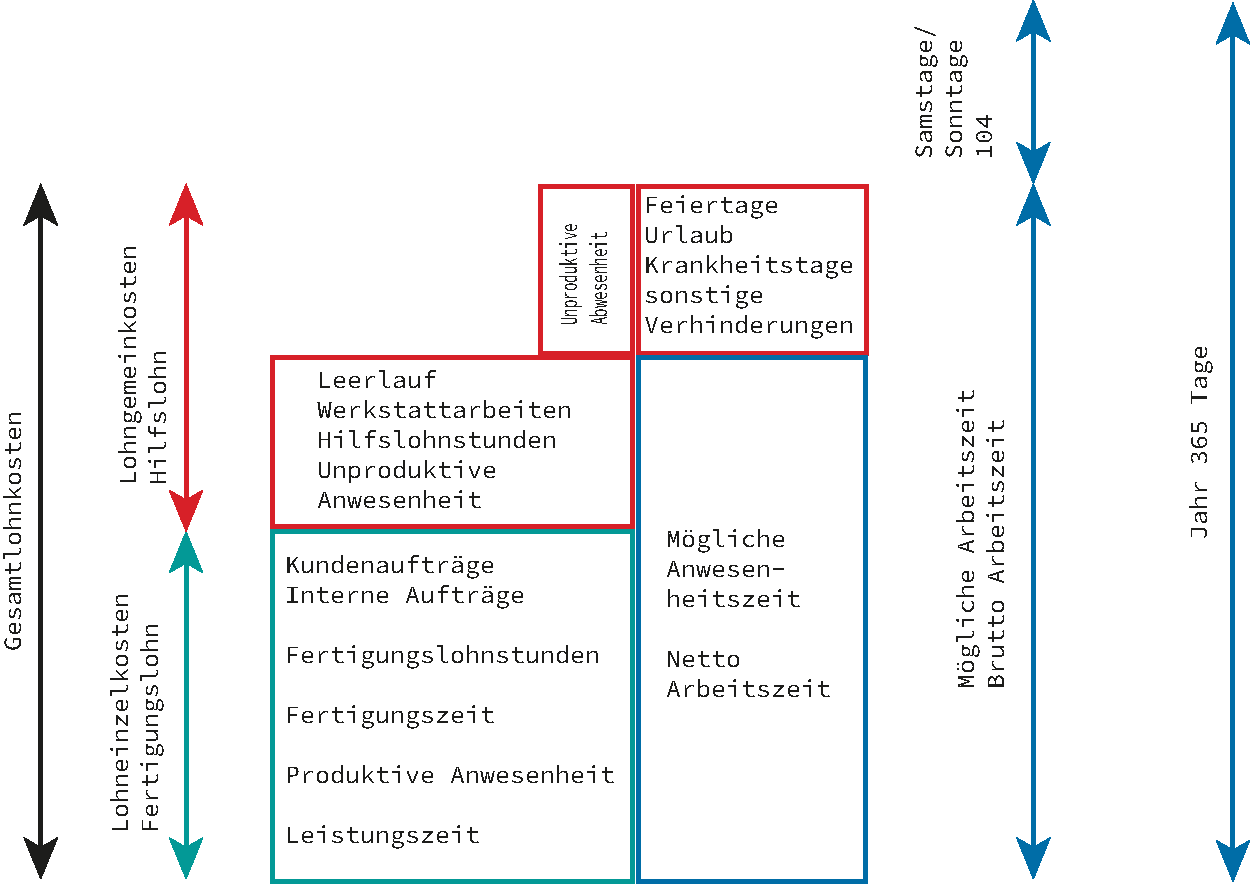
\includegraphics[width=0.9\textwidth]{images/Skizze/Arbeitszeitermittlung.pdf}
\caption{Arbeitszeitermittlung}
%\label{fig:}%% anpassen
\end{figure}

\textbf{Ermittlungsschema}

\lstset{language=Bash}% C, TeX, Bash, Python 
\begin{lstlisting}[
	%caption={}, label={code:}%% anpassen
]
  Kalendertage pro Jahr                              365
- Samstag/Sonntag (5-Tage-Woche, 52 x 2)             104
= Mögliche Arbeitszeit (Brutto)                      261
- Feiertage (je Bundesland)                            9
- Urlaubstage (min. 24 Werktage)                      29
- Krankheitstage                                       8
- Schulungstage                                        6 
= Mögliche Anwesenheitstage (Netto)                  209
  Tägliche Arbeitszeit 8 h 
_____________________________________________________________
= Mögliche Anwesenheitszeit in Stunden (209 x 8 h) 1.672 h
  Leistungszeit (produktive Arbeitszeit)
  Leerlauf      (unproduktive Arbeitszeit)
_____________________________________________________________
= Arbeitstage pro Jahr (261 - Feiertage)             252 Tage
\end{lstlisting}

\textbf{Werktag} (Mo. - Sa.)

\newpage

\section{Serviceberater - Kundendienstberater -
Dialogannahme}\label{serviceberater-kundendienstberater-dialogannahme}

\textbf{Skript - Serviceberater}

\begin{itemize}
\item
  >>Mädchen für alles<<
\item
  Vollzeitjob, hat viele Einsatzmöglichkeiten
\item
  Im Durchschnitt 8 bis 14 Kunden pro Tag
\item
  Small Talk halten: Wieso, Weshalb, Warum?
\item
  Das kleine 1x1 des Serviceberaters
\end{itemize}

\textbf{Vorgehensweise des KD-Beraters bei der Auftragsannahme}

\begin{itemize}
\item
  Fragen nach dem Kundenwunsch
\item
  Durchführung der Untersuchung des Fahrzeuges
\item
  Dokumentation von Schäden am Fahrzeug
\item
  Erfassung von Wertgegenständen im Fahrzeug
\item
  Probefahrt mit dem Kunden
\item
  Mitteilung des kalkulierten Preises
\item
  Auftrag erstellen
\end{itemize}

\textbf{Bereiche des Autohauses, die an der Bearbeitung des Auftrags
beteiligt sind?}

\begin{enumerate}
\item
  \textbf{Annahme Kundendienst}

  \begin{itemize}
  \item
    \emph{Aufgaben} Annahme von Reparaturen, technische Beratung des
    Kunden, Fahrzeugübergabe
  \end{itemize}
\item
  \textbf{Werkstatt}

  \begin{itemize}
  \item
    \emph{Aufgaben} Durchführung von Reparaturen und Wartungsarbeiten
  \end{itemize}
\item
  \textbf{Teiledienst}

  \begin{itemize}
  \item
    \emph{Aufgaben} Verwaltung von den Ersatzteilen und Zubehör, Ausgabe
    von Teilen, Verkauf von Teilen
  \end{itemize}
\item
  \textbf{Verkauf}

  \begin{itemize}
  \item
    \emph{Aufgaben} Kundenberatung
  \end{itemize}
\item
  \textbf{Verwaltung}

  \begin{itemize}
  \item
    \emph{Aufgaben} Zahlungserinnerung einer nicht gezahlten Rechnung an
    den Kunden
  \end{itemize}
\item
  \textbf{Geschäftsleitung}

  \begin{itemize}
  \item
    \emph{Aufgaben} Kundenbeschwerde über eine zu hohe Rechnung
  \end{itemize}
\end{enumerate}

\textbf{Vorteile Direktannahme}

\begin{itemize}
\item
  Möglichkeit zur Kommunikation mit dem Kunden schaffen
\item
  über Mängel sofort informieren
\item
  Missverständnisse können vermieden werden
\item
  Rückfragen werden verringert
\item
  teure Reparatur erkennen vs.~Zeitwert / Wiederbeschaffungswert $\to$
  zeitwertgerechte Reparatur
\item
  günstige Ersatzteile oder Gebrauchtteile $\to$ verkehrstüchtigen
  Zustand
\item
  bei sicherheitsrelevanten Mängel $\to$ nicht mehr fahren lassen!
  (Polizei informieren bei hartnäckigen Fällen)
\item
  Entscheidend ist kompetente Person oder Schnarchnase!
\end{itemize}

\section{Auftragsabwicklung und
Kundenservice}\label{auftragsabwicklung-und-kundenservice}

Vgl. Auftragsabwicklung Fachbuch S. 149-158
(\textcite{heiser:2017:betriebsfuhrung}).

\textbf{Arbeitsplanung - Auftragsannahme bis Fahrzeugrückgabe}

\begin{enumerate}
\item
  \textbf{Terminvereinbarung} Auftragsannahme

  \begin{itemize}
  \item
    Termin mit Kunden vereinbaren, Terminvorbereitung
  \end{itemize}
\item
  \textbf{Terminvorbereitung}

  \begin{itemize}
  \item
    KD-Berater plant Fahrzeugdurchsicht auf Basis Fahrzeughistorie
  \end{itemize}
\item
  \textbf{Fahrzeugannahme}

  \begin{itemize}
  \item
    Fahrzeug wird vom KD-Berater übernommen und Fahrzeugcheck
    durchgeführt
  \end{itemize}
\item
  \textbf{Auftragserstellung}

  \begin{itemize}
  \item
    notwendige Arbeiten erfassen und Werkstattauftrag erstellen
  \item
    Teileverfügbarkeit prüfen
  \end{itemize}
\item
  \textbf{Reparatur}

  \begin{itemize}
  \item
    In der Werkstatt wird nach Herstellervorgaben des Fahrzeug instand
    gesetzt
  \end{itemize}
\item
  \textbf{Qualitätskontrolle}

  \begin{itemize}
  \item
    Ausführung der Arbeit überprüfen, Endkontrolle / Sichtkontrolle /
    Probefahrt
  \end{itemize}
\item
  \textbf{Vorbereiten der Fahrzeugrückgabe}

  \begin{itemize}
  \item
    Rückgabe vorbereiten und Rechnung erstellen, Rechnung prüfen
  \end{itemize}
\item
  \textbf{Fahrzeugrückgabe}

  \begin{itemize}
  \item
    Fahrzeug an Kunde übergeben und Arbeiten anhand der Rechnung
    erläutern, Kunde zahlt Rechnung
  \end{itemize}
\item
  \textbf{Nachbearbeitung}

  \begin{itemize}
  \item
    Kundenzufriedenheit prüfen anhand von Nachfragen
  \item
    anonymer Fragebogen (telefonisch, Internet, Post)
  \end{itemize}
\end{enumerate}

\textbf{Organigramm} $\to$ Hierarchisch strukturiert,
Organisationsstruktur, Weisungsbeziehungen

\textbf{Softskills} $\to$ Selbstsicherheit, Selbstständigkeit,
Entscheidungsfähigkeit

\section{Betriebsorganisation}\label{betriebsorganisation}

Das Ziel ist, Gewinn zu erzielen. Dies wird erreicht durch den optimalen
Einsatz von Mitarbeitern, Maschinen, Material und Zeit.

\textbf{Maximalprinzip}: Mit gegebenen Mitteln eine möglichst hohe
Leistung erzielen. \textbf{Minimalprinzip}: Eine vorbestimmte Leistung
mit möglichst geringen Mitteln erzielen.

\textbf{Kundenorientierung} ist die Ausrichtung des Denkens und Handelns
der Mitarbeiter auf den Kunden und seine Bedürfnisse. Macht das
wirtschaftlich Sinn?

\textbf{Was beeinflusst die Kundenzufriedenheit? Nenne Merkmale}

\begin{itemize}
\item
  \textbf{Technische Produktqualität}

  \begin{itemize}
  \item
    Verarbeitung und Reparaturanfälligkeit
  \item
    Ausführung von Wartungs- und Reparaturarbeiten
  \end{itemize}
\item
  \textbf{Servicequalität}

  \begin{itemize}
  \item
    Kulanzregelungen
  \item
    Einhaltung von Terminen
  \item
    Qualität der Beratung
  \item
    Umgang mit Reklamationen an
  \end{itemize}
\item
  Reputationsqualität

  \begin{itemize}
  \item
    Guter Ruf, Kompetenz
  \end{itemize}
\item
  Persönliche Beziehungsqualität

  \begin{itemize}
  \item
    Mitarbeiter - Kunde
  \end{itemize}
\item
  Preiswahrnehmung

  \begin{itemize}
  \item
    Gutes Preis-Leistungs-Verhältnis, Angebote, Transparenz
  \end{itemize}
\item
  Kundenbindung

  \begin{itemize}
  \item
    Ziel: langfristige Bindung
  \end{itemize}
\end{itemize}

\textbf{Servicekonzepte, die Kundenbindung verbessern}

\begin{itemize}
\item
  Werbung
\item
  Garantie und Kulanz
\item
  Hol- und Bring-Service
\item
  Reparatur-Finanzierung
\item
  Dienstleistungsangebote: Verkauf, Wartung
\end{itemize}

Bestandskunden halten vs.~Neukunden bewerben kostet 5-6x mehr

\textbf{Kundenarten}

\begin{itemize}
\item
  \textbf{Laufkunde} (Kommt zufällig und hat keine Bindung)

  \begin{itemize}
  \item
    \emph{Bedeutung} Gering
  \item
    \emph{Erwartung des Kunden} Schnelle und zuverlässige Ausführung der
    Arbeit
  \item
    \emph{Maßnahmen} Keine
  \end{itemize}
\item
  \textbf{Dauerkunde} (nimmt gelegentlich Service in Anspruch)

  \begin{itemize}
  \item
    \emph{Bedeutung} Mittel
  \item
    \emph{Erwartung des Kunden} zuverlässig und preisgünstig
  \item
    \emph{Maßnahmen} Angebote an Kunden
  \end{itemize}
\item
  \textbf{Stammkunde} (lässt alle Arbeiten in der Werkstatt ausführen)

  \begin{itemize}
  \item
    \emph{Bedeutung} Hoch
  \item
    \emph{Erwartung des Kunden} persönliche Betreuung
  \item
    \emph{Maßnahmen} persönliche Ansprache
  \end{itemize}
\item
  \textbf{Großkunde} (Gesamten Fuhrpark warten)

  \begin{itemize}
  \item
    \emph{Bedeutung} sehr hoch
  \item
    \emph{Erwartung des Kunden} Schnelle und gute Ausführung, Kulanz
  \item
    \emph{Maßnahmen} Rabatt, Terminvereinbarung
  \end{itemize}
\end{itemize}

\emph{Vorsicht bei Zahlungszielen} von 30 oder 60 Tage Z. B. Aldi legt
bei einer Bank stundenweise / 28 Tage lang Geld an und lässt das Geld
für sich arbeiten.

\section{Reklamation und Umtausch}\label{reklamation-und-umtausch}

\textbf{Reklamationen} sind nicht erfüllte Kundenerwartungen

\begin{itemize}
\item
  Kundenbedürfnisse herausfinden
\item
  kundenorientierte Lösung anbieten (Kulanz bei einem guten Kunden)
\item
  bei Kundenzufriedenheit kommen Kunden wieder
\end{itemize}

\textbf{Umtausch} geht es um die Rücknahme eines fehlerfreien Produktes

\textbf{Kundenreklamation}

\begin{itemize}
\item
  \emph{Beschwerden als Chance sehen}
\item
  Reklamationsmanagement hilft bei der Kundenbindung
\item
  Beschwerden anregen (Beispiel Fragebögen)
\item
  \emph{Valide} Aussagekräftig
\item
  Wirtschaftspsychologe werten Fragebögen aus
\item
  Kontrollmechanismus einbauen -- kommt die Beschwerde auch an?
\end{itemize}
